%%%%%%%%%%%%%%%%%%%% book.tex %%%%%%%%%%%%%%%%%%%%%%%%%%%%%
%
% sample root file for the chapters of your "monograph"
%
% Use this file as a template for your own input.
%
%%%%%%%%%%%%%%%% Springer-Verlag %%%%%%%%%%%%%%%%%%%%%%%%%%


% RECOMMENDED %%%%%%%%%%%%%%%%%%%%%%%%%%%%%%%%%%%%%%%%%%%%%%%%%%%
\documentclass[envcountsame,envcountchap]{svmono}

% choose options for [] as required from the list
% in the Reference Guide, Sect. 2.2
\usepackage{geometry} 
\usepackage{makeidx}         % allows index generation
\usepackage{graphicx}        % standard LaTeX graphics tool
                             % when including figure files
\usepackage{multicol}        % used for the two-column index
\usepackage[bottom]{footmisc}% places footnotes at page bottom
\usepackage[italian]{babel}
\usepackage[utf8]{inputenc}

\usepackage{amsmath}%  %
\usepackage{amsfonts}%
\usepackage{amssymb}%es
\usepackage{mathtools}

\usepackage{hyperref}
\hypersetup{colorlinks=true, linkcolor=black} %per colorare i link

\DeclarePairedDelimiter{\abs}{\lvert}{\rvert}
\DeclarePairedDelimiter{\norma}{\lVert}{\rVert}

% etc.
% see the list of further useful packages
% in the Reference Guide, Sects. 2.3, 3.1-3.3

\makeindex             % used for the subject index
                       % please use the style svind.ist with
                       % your makeindex program


%%%%%%%%%%%%%%%%%%%%%%%%%%%%%%%%%%%%%%%%%%%%%%%%%%%%%%%%%%%%%%%%%%%%%

\begin{document}

\author{Roberto Melfi}
\title{Pattern Classification Lecture Notes\\
{\small Pattern Classification Course - A.Y. 2008/2009}}
\subtitle{In Memory of Prof. Alfredo Petrosino}
\maketitle

\frontmatter%%%%%%%%%%%%%%%%%%%%%%%%%%%%%%%%%%%%%%%%%%%%%%%%%%%%%%


%%%%%%%%%%%%%%%%%%%%%%% dedic.tex %%%%%%%%%%%%%%%%%%%%%%%%%%%%%%%%%
%
% sample dedication
%
% Use this file as a template for your own input.
%
%%%%%%%%%%%%%%%%%%%%%%%% Springer-Verlag %%%%%%%%%%%%%%%%%%%%%%%%%%

\thispagestyle{empty}
\vspace*{3.5cm}
\begin{flushright}

% write your text here
{\large Your dedication goes here}

\end{flushright}




%%%%%%%%%%%%%%%%%%%%%% pref.tex %%%%%%%%%%%%%%%%%%%%%%%%%%%%%%%%%%%%%
%
% sample preface
%
% Use this file as a template for your own input.
%
%%%%%%%%%%%%%%%%%%%%%%%% Springer-Verlag %%%%%%%%%%%%%%%%%%%%%%%%%%

\preface

%% Please write your preface here
Questi appunti sono stati scritti durante il corso di Riconoscimento e Classificazione di Forme tenuto dal Professore Alfredo Petrosino nell’anno accademico 2008/2009. Non sono semplici appunti, ma un’accurata sbobinatura di registrazioni delle sue lezioni unite a parti tradotte e sintetizzate del libro “Duda Hart” \cite{duda}. 
A distanza di circa dieci anni rendo pubblico questo lavoro, non per meriti, ma per tramandare per iscritto le lezioni del professore ai futuri studenti, se esistono questi appunti è solo grazie al suo corso, ho avuto soltanto la pazienza di trascriverli e organizzarli per poter preparare al meglio l’esame finale. \\
Gli appunti sono open source (\url{https://github.com/robmelfi/PatternRecognitionLectureNotes}), cosi da correggere eventuali errori di battitura e migliorare parti non abbastanza curate da parte mia. 
Il professore ha insegnato che la perfezione non esiste, ma un lavoro può essere sempre migliorato per tendere alla perfezione, questi appunti devono essere un punto di partenza per essere ampliati lasciando inalterate e mettendo in evidenza le parole del professore. 



%% Please "sign" your preface

\begin{flushright}\noindent
\hfill {\it Roberto Melfi}\\
\end{flushright}

\vspace{1cm}
\noindent Il ruolo di un professore è quello di essere guida e di insegnare la vita, oltre che la disciplina.
Gli studenti dell’Università Parthenope che hanno conosciuto il professore Alfredo Petrosino possono dire di aver avuto un’insegnante che ha ricoperto a pieno questo ruolo.
Grazie a lui abbiamo creato un gruppo di studio tra le scrivanie del CVPRLab che andava oltre i banchi universitari.
Durante tutto il percorso accademico abbiamo trascorso dei momenti intensi che ci han forgiato rendendoci le persone migliori che siamo oggi. Non gli saremo mai abbastanza riconoscenti per questo!
La sua prematura scomparsa è stata un fulmine a ciel sereno che ha riunito sotto lo stesso tetto, tutte le persone che lo conoscevano ed avevano lavorato con lui. Anche in questo momento è stato speciale dato ci siamo riuniti dopo anni in cui ognuno di noi ha intrapreso la sua strada.
Grazie di tutto prof!\\

“ti aspetterò comunque fruori alla porta 429 ... sarai semplicemente in ritardo ...”, il saluto di un suo caro allievo \emph{Enrico Balestrieri}.

\begin{flushright}\noindent
\hfill {\it Luca Russo}\\
\end{flushright}

\vspace{0.5cm}
Napoli, Gennaio 2020







\tableofcontents


\mainmatter%%%%%%%%%%%%%%%%%%%%%%%%%%%%%%%%%%%%%%%%%%%%%%%%%%%%%%%
%%%%%%%%%%%%%%%%%%%%%%%% part.tex %%%%%%%%%%%%%%%%%%%%%%%%%%%%%%%%%%
%
% sample part title
%
% Use this file as a template for your own input.
%
%%%%%%%%%%%%%%%%%%%%%%%% Springer-Verlag %%%%%%%%%%%%%%%%%%%%%%%%%%


\part{Parte Uno}

%%%%%%%%%%%%%%%%%%%%% chapter.tex %%%%%%%%%%%%%%%%%%%%%%%%%%%%%%%%%
%
% sample chapter
%
% Use this file as a template for your own input.
%
%%%%%%%%%%%%%%%%%%%%%%%% Springer-Verlag %%%%%%%%%%%%%%%%%%%%%%%%%%

\chapter{Bayesian Decision Theory}\label{teoriaBaesiana}
\label{teoriaBaesiana} % Always give a unique label
% use \chaptermark{}
% to alter or adjust the chapter heading in the running head

\section{Introduzione}
La Teoria delle decisioni baesiane è un fondamentale approccio statistico per il problema del \emph{Pattern Classification}. L'esempio preso in considerazione è quello di progettare un classificatore  che sia in grado di separare due specie di pesci: il branzino ed il salmone. Supponiamo che ci sia un operatore che sta osservando un nastro trasportatore sul quale scorrono queste due specie, l'osservatore trova difficile predire quale specie si presenterà all'arrivo del prossimo pesce. Denotiamo con $\omega$ lo \textbf{stato della natura}, poniamo $\omega = \omega_1$ per il branzino e $\omega = \omega_2$ per il salmone. Poichè lo stato della natura è imprevedibile allora consideriamo $\omega$ una variabile che deve essere descritta probabilisticamente. Si assume che siamo a conoscenza delle \textbf{probabilità a priori}, denotiamo con $P(\omega_1)$ la probabilità che il prossimo pesce sia un branzino e con $P(\omega_2)$ la probabilità che il prossimo pesce sia un salmone, se si assume che non ci siano altre tipologie di pesci allora la somma di $P(\omega_1)$ e $P(\omega_2)$ è uguale ad uno. Le due probabilità possono essere ricavate statisticamente sulla storia passata, quindi una regola di decisione potrebbe essere quella di scegliere $\omega_1$ se $P(\omega_1) > P(\omega_2)$, altrimenti viene scelto $\omega_2$. Questa regola potrebbe avere senso se prendiamo in considerazione soltanto due tipologie di classi, infatti potrebbe risultare strano se si applica questa regola quando c'è da classificare più di due classi. Nella maggior parte delle circostanze non è utile prendere decisioni con così poche informazioni. Nella classificazione tra le due specie di pesci, per esempio possiamo prendere in considerazione la misura della luminanza
$x$ per migliorare il nostro classificatore. Ogni pesce avrà una luminanza diversa ed è possibile esprimere questa variabile in termini probabilistici, si considera $x$ come una variabile casuale la cui distribuzione dipende dallo stato della natura ed è espressa come $p(x|\omega)$ che viene definita funzione della densità di probabilità condizionale, ovvero la funzione della densità di probabilità per $x$ dato lo stato della natura $\omega$. Quindi la differenza tra $p(x|\omega_1)$ e  $p(x|\omega_2)$ descrive la differenza di luminanza tra la popolazione dei branzini e quella dei salmoni (fig. \ref{cpdf}).


\begin{figure}
\centering
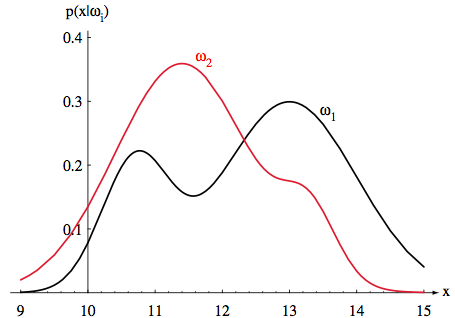
\includegraphics[scale=0.6]{img/cpdf.png}
\caption{Funzione di densità della probabilità condizionate delle due classi di pesci per la caratteristica della luminanza $x$}
\label{cpdf}
\end{figure}
\noindent Supponiamo che siamo a conoscenza di entrambi le probabilità a priori $P(\omega_j)$ e delle funzioni di densità della probabilità condizionata $p(x|\omega_j)$ per $j = 1,2$. Supponiamo che arrivi un pesce sul nastro trasportatore e misuriamo la luminanza $x$. Qui entra in gioco la regola di Bayes. Conosciamo $p(x|\omega_j) = p(x \cap \omega_j) / P(\omega_j)$, il nostro obiettivo è quello di calcolare $P(\omega_j | x)$, ovvero la probabilità di appartenenza alla classe $\omega_j$ dato la misura di luminanza $x$ rilevata. $P(\omega_j | x) = P(x \cap \omega_j) / p(x)$, quindi per il teorema della moltiplicazione
\begin{gather}
p(\omega_j \cup x) = p(x|\omega_j) P(\omega_j)\\
p(\omega_j \cup x) = P(\omega_j|x ) p(x)
\end{gather}
riarrangiando i termini otteniamo la risposta al nostro quesito mediante la regola di Bayes
\begin{equation}
P(\omega_j|x) = \frac{p(x|\omega_j) P(\omega_j)}{p(x)}
\end{equation}
dove nel caso di due categorie
\begin{equation}
p(x) = \sum_{j=1}^2 p(x|\omega_j) P(\omega_j)
\end{equation}
La formula di Bayes può essere espressa informalmente  dicendo che
\begin{equation}
\text{Posterior} = \frac{\text{likelihood (verosomigianza)} \times \text{prior}}{\text{evicence}}
\end{equation}
La formula di Bayes mostra che osservando il valore di $x$ possiamo convertire la \textbf{probabilità a priori} $P(\omega_j)$ nella \textbf{probabilità a posteriori} $P(\omega_j|x)$, ovvero la probabilità di avere la classe $\omega_j$ dato il valore $x$ misurato. Chiamiamo $P(x|\omega_j)$ \emph{\textbf{likelihood}} (verosomiglianza) di $\omega_j$ rispetto ad $x$. $p(x)$ invece è il fattore evidenza e può essere visto come un fattore di scala che garantisce che la somma delle probabilità a posteriori sia uguale ad uno. La variazione di $P(\omega_j|x)$ è illustrata in figura \ref{prob_post} per il caso con $P(\omega_1) = 2/3$ e $P(\omega_2) = 1/3$.
\begin{figure}
\centering
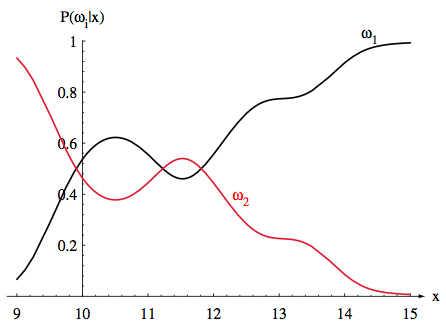
\includegraphics[scale=0.6]{img/prob_post.png}
\caption{Probabilità posteriori calcolate per le probabilità a priori $P(\omega_1) = 2/3$ e $P(\omega_2) = 1/3$ per le funzioni di densità di probabliità condizionata mostrate in fig. \ref{cpdf}}
\label{prob_post}
\end{figure}
\noindent Quindi nel caso di due classi è ovvio scegliere $\omega_1$ se $P(\omega_1|x) > P(\omega_2|x)$ e viceversa. Per giustificare questa procedura di decisione è opportuno calcolare la probabilità di errore. Qualsiasi sia la variabile $x$ osservata la probabilità di errore è

\[
P(error | x)=
\begin{cases}
P(\omega_1|x) & \text{se dicidiamo $\omega_2$} \\
P(\omega_2|x) & \text{se dicidiamo $\omega_1$} 
\end{cases}
\]


\section{Teoria delle decisioni baesiane -- Continuous Features}

In questo paragrafo verrà formalizzata l'idea descritta nel paragrafo precedente e viene generalizzata in modo tale da 
\begin{itemize}
\item Consentire l'uso di più caratteristiche
\item Consentire la classificazione tra più classi
\item Consentire l'esecuzione di altre azioni semplicemente decidendo lo stato della natura
\item Introducendo una funzione di perdita più generale della probabilità d'errore
\end{itemize}
Per quanto riguarda il primo punto basta semplicemente sostituire lo scalare $x$ con un \emph{feature vector} (vettore delle caratteristiche) $\mathbf{x}$, dove $\mathbf{x}$ è un vettore a $d$ dimensioni nello spazio Euclideo 	$\mathbf{R}^d$, chiamato \emph{feature space} (spazio delle carateristiche), quindi analogamente al caso precedente denotiamo con $p(\mathbf{x}|\omega_j)$ la funzione di densità della probabilità condizionata per $\mathbf{x}$. Come prima, $P(\omega_j)$ descrive la probabilità a priori per le varie classi $\omega_j$, quindi la probabilità a posteriori può essere ottenuta mediante la formula di Bayes:
\begin{equation}
P(\omega_j| \mathbf{x}) = \frac{p(\mathbf{x}|\omega_j) P(\omega_j)}{p(\mathbf{x})}
\end{equation}
in questo caso l'evidenza viene calcolata come segue
\begin{equation}
p(x) = \sum_{j=1}^c p(\mathbf{x} | \omega_j) P(\omega_j)
\end{equation}
Le formule appena descritte possono essere utilizzate anche per estendere la classificazione tra $c$ classi.\\

\noindent In generale classificare significa anche prendere una decisione dell'azione da intraprendere. Denotiamo con $\{\omega_1, \dots, \omega_c\}$ un insieme finito di $c$ categorie e con $\{\alpha_1, \dots, \alpha_a\}$ un insieme finito di $a$ possibili azioni da intraprendere, inoltre denotiamo con $\lambda(\alpha_i|\omega_j)$ la funzione di perdita che descrive la perdita o il costo al quale si incorre nel caso venga scelta l'azione $\alpha_i$ quando si è scelta la classe $\omega_j$. Possiamo definire \emph{rischio} la perdita $R(\alpha_i|\mathbf{x})$, ovvero la perdita che si ha nel caso si sia scelto di eseguire l'azione $\alpha_i$ dato il vettore delle caratteristiche $\mathbf{x}$ e viene calcolata come segue
\begin{equation}\label{risk}
R(\alpha_i | \mathbf{x}) = \sum_{j=1}^c \lambda(\alpha_i | \omega_j) P(\omega_j | \mathbf{x})
\end{equation}
Qualunque sia l'osservazione $\mathbf{x}$, è possibile minimizzare la perdita selezionando l'azione che minimizza il rischio. Un problema è quello di trovare una regola di decisione che minimizza il rischio totale. Una regola di decisione generale è la funzione $\alpha(\mathbf{x})$ che ci dice quale azione eseguire per ogni possibile osservazione. Quindi per ogni osservazione $\mathbf{x}$ è associata un unica azione $\alpha_1, \dots, \alpha_a$. Il rischio associato ad una data regola di decisione misura la perdita attesa quando tale regola venisse adottata su tutte le osservazioni $\mathbf{x}$
\begin{equation}
R = \int R(\alpha(\mathbf{x}) | \mathbf{x}) p(\mathbf{x}) \ d\mathbf{x}
\end{equation}
per minimizzare il rischio totale allora si calcolano tutti i rischi $R(\alpha_i | \mathbf{x})$ per $i=1, \dots, a$ e si sceglie l'azione $\alpha_i$ per la quale il rischio $R(\alpha_i | \mathbf{x})$ è minimo.

\subsection{Classificazione tra due categorie}
Consideriamo un problema di classificazione tra soltanto due categorie. Quindi abbiamo l'azione $\alpha_1$ che corrisponde alla decisione presa se il classificatore da come risultato $\omega_1$ e l'azione $\alpha_2$ che corrisponde alla decisione presa se il classificatore restituisce $\omega_2$. Per semplificare la notazione poniamo la funzione di perdita $\lambda_{ij} = \lambda(\alpha_i, \omega_j)$, che come abbiamo detto corrisponde alla perdita nel caso si esegue l'azione $\alpha_i$ scelta la categoria $\omega_j$. Dall'equazione \ref{risk} otteniamo il rischio
\begin{gather}
R(\alpha_1 | \mathbf{x}) =  \lambda_{11} P(\omega_1 | \mathbf{x}) + \lambda_{12} P(\omega_2 | \mathbf{x})\\
R(\alpha_2 | \mathbf{x}) =  \lambda_{21} P(\omega_1 | \mathbf{x}) + \lambda_{22} P(\omega_2 | \mathbf{x})
\end{gather}
Ci sono molti metodi per esprimere la regola di decisione del minimo rischio. La regola fondamentale è quella di decidere $\omega_1$ se $R(\alpha_1 | \mathbf{x}) < R(\alpha_2 | \mathbf{x})$. Invece in termini di probabilità a posteriori otteniamo da semplici sostituzioni la seguente regola decidendo $\omega_1$ se
\begin{equation}
(\lambda_{21} - \lambda_{11}) P(\omega_1 | \mathbf{x}) > (\lambda_{12} - \lambda_{22}) P(\omega_2 | \mathbf{x})
\end{equation}
 Invece, utilizzando la regola di Bayes possiamo sostituire le probabilità a posteriori con le probabilità a priori e le funzioni di densità di probabilità condizionata, ciò equivale a decidere $\omega_1$ se
\begin{equation}
(\lambda_{21} - \lambda_{11}) p(\mathbf{x}|\omega_1) P(\omega_1) > (\lambda_{12} - \lambda_{22}) p(\mathbf{x}|\omega_2) P(\omega_2)
\end{equation}
Un altra alternativa, assumendo $\lambda_{21} > \lambda_{11}$, è quella di decidere $\omega_1$ se
\begin{equation}
\frac{p(\mathbf{x}|\omega_1)}{p(\mathbf{x}|\omega_2)} > \frac{\lambda_{12} - \lambda_{22}}{\lambda_{21} - \lambda_{11}} \ \frac{P(\omega_2)}{P(\omega_1)}
\end{equation}
Questa regola di decisione si focalizza sulla dipendenza $\mathbf{x}$ dalla densità della probabilità condizionate. Possiamo considerare $p(\mathbf{x}|\omega_1) / p(\mathbf{x}|\omega_2)$ il rapporto di verosomiglianza (\emph{likelihood ratio}). Questa regola di decisione baesiana può essere utilizzata per decidere $\omega_1$ se il tasso di verosomiglianza supera una determinata soglia rendendo così la regola indipendente dall'osservazione $\mathbf{x}$

\section{Classificazione con tasso di errore minimo}
Nel problema della classificazione ogni stato è generalmente associato ad una classe, e l'azione $\alpha_i$ viene associata allo stato $\omega_i$. In generale se l'azione è $\alpha_i$ e lo stato è $\omega_j$ allora la decisione è corretta se $i = j$ ed è sbagliata se $i \neq j$. Per evitare gli errori allora è opportuno cercare regole di decisione che minimizzano gli errori o tasso di errore (\emph{error rate}). La funzione di perdita in questo caso è chiamata simmetrica o funzione di perdita \emph{zero-one},
\[
\lambda(\alpha_i, \omega_j)=
\begin{cases}
0 & \text{se} \ i = j\\
1 & \text{se} \ i \neq j 
\end{cases} 
\quad \quad \quad
i,j = 1, \dots, c.
\]
Questa funzione non assegna perdita ad una decisione corretta mentre assegna una perdita pari a uno quando la decisione è sbagliata. Il rischio quindi è calcolato come segue
\begin{equation}
\begin{split}
R(\alpha_i | \mathbf{x}) &= \sum_{j=1}^c \lambda(\alpha_i | \omega_j ) P(\omega_j | \mathbf{x}) \\
&= \sum_{j \neq i} P(\omega_j | \mathbf{x})\\
&= 1 - P(\omega_i | \mathbf{x})
\end{split}
\end{equation}
Quindi per minimizzare il tasso di errore dobbiamo scegliere l'indice $i$ che massimizza la probabilità a posteriori (MAP) $P(\omega_i | \mathbf{x})$. In altre parole per il tasso di errore minimo decidiamo $\omega_i$ se
\begin{equation}
P(\omega_i | \mathbf{x}) > P(\omega_j | \mathbf{x}) \quad \quad \quad \text{per tutti} \quad  j \neq i
\end{equation}

\section{Classificatori, Funzioni discriminanti e superfici di decisione}
\subsection{Il caso multicategoria}\label{casoMulticategoria}
Ci sono tanti modi diversi per rappresentare un classificatore di pattern. Uno dei più comunemente usati si basa sulle \emph{funzioni discriminanti} $g_i(\mathbf{x}), \ i = 1, \dots, c.$ Il classificatore ci dice di assegnare il vettore delle caratteristiche $\mathbf{x}$ alla classe $\omega_j$ se
\begin{equation}
g_i(\mathbf{x}) > g_j(\mathbf{x}) \ \ \ \text{per ogni} \ j \neq i
\end{equation}
Il classificatore può essere visto come una rete di macchine che calcolano le $c$ funzioni discriminanti e sceglie la categoria corrispondente alla funzione discriminante che ha restituito una risposta maggiore.
\begin{figure}
\centering
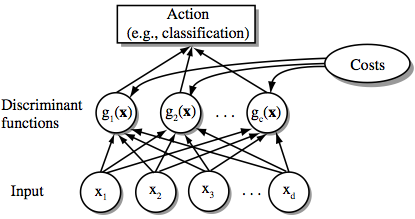
\includegraphics[scale=0.7]{img/network.png}
\caption{La struttura funzionale di comune classificatore di pattern la quale include $d$ input e $c$ funzioni discriminanti $g_i(\mathbf{x})$. Viene determinato quale dei valori discriminanti è il massimo e viene classificato il pattern di input.}
\label{network}
\end{figure}
In figura \ref{network} possiamo osservare un classificatore basato su una rete di funzioni discriminanti.
Un classificatore Baesiano  è semplicemente e naturalmente rappresentato in questo modo. Per un caso più generale, dove viene preso in considerazione anche il rischio, possiamo dire che $g_i(\mathbf{x}) = -R(\alpha_i|\mathbf{x})$, poiché la funzione discriminante massima corrisponde al minimo rischio. Invece per il caso a minimo tasso di errore possiamo semplificare ulteriormente le cose considerando $g_i(\mathbf{x}) = P(\omega_i|\mathbf{x})$, in questo modo affermiamo che la funzione discriminante massima corrisponde alla massima probabilità a posteriori (MAP). La scelta della funzione discriminante non è unica, è possibile moltiplicare tutte le funzioni discriminanti con una costante positiva senza influenzare la decisione. Inoltre, se sostituiamo ogni $g_i(\mathbf{x})$ con $f(g_i(\mathbf{x}))$, dove $f(\cdot)$ è una funzione monotona crescente, il risultato della classificazione resta invariato. Questa osservarzione comporta il vantaggio di significative semplificazioni analitiche e computazionali. In particolare, per la classificazione a tasso minimo di errore, qualsiasi delle seguenti scelte danno la stessa risposta di classificazione, ma alcune possono risultare più semplici da capire o da calcolare rispetto alle altre:
\begin{gather}
g_i(\mathbf{x}) = P(\omega_i|\mathbf{x}) = \frac{p(\mathbf{x}|\omega_i) P(\omega_i)}{\sum_{j=1}^c p(\mathbf{x} | \omega_j) P(\omega_j)}\\
g_i(\mathbf{x}) = p(\mathbf{x}|\omega_i) P(\omega_i)\\
g_i(\mathbf{x}) = \ln p(\mathbf{x}|\omega_i) + \ln P(\omega_i)
\end{gather} 
dove con $\ln$ indichiamo il logaritmo naturale.
Come abbiamo visto le funzioni discriminanti possono essere descritte in vari modi ma le regole di decisione sono equivalenti. Lo scopo di qualsiasi regola di decisione è quello di dividere lo spazio delle caratteristiche in $c$ \emph{regioni di decisione}, $\mathcal{R}_1, \dots, \mathcal{R}_c$. Se $g_i(\mathbf{x}) > g_j(\mathbf{x})$ per ogni $j \neq i$, allora $\mathbf{x}$ è in $\mathcal{R}_i$ e la regola di decisione assegna $\mathbf{x}$ a $\omega_i$. Le regioni sono separate dai \emph{decision boundaries} che possiamo osservare in fig. \ref{decisionBoundaries}
\begin{figure}
\centering
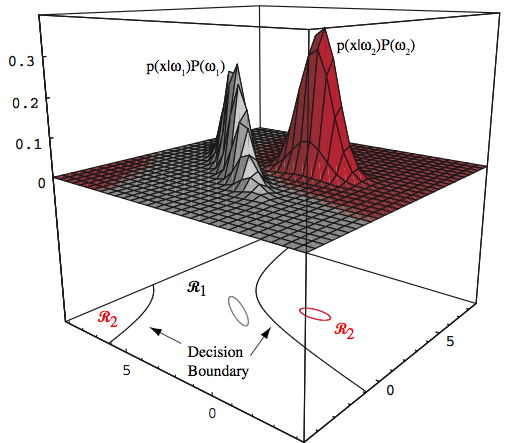
\includegraphics[scale=0.6]{img/decisionBoundaries.png}
\caption{Classificatore tra due categoria in due dmensioni, le densità di probabilità sono gaussiane, i bordi di decisione consistono in due iperbole e la regione di decisione $\mathcal{R}_2$ non è semplicemente connessa}
\label{decisionBoundaries}
\end{figure}

\subsection{Il caso a due categorie}
Il caso a due categorie è un caso speciale del caso multigategoria, e riceve un trattamento separato. Prende anche il nome speciale \emph{dichotomizer}. Invece di usare le due funzioni discriminanti $g_1$ e $g_2$ e assegnare $\mathbf{x}$ a $\omega_1$ se $g_1 > g_2$, è comune definire una singola funzione discriminante 
\begin{equation}
g(\mathbf{x}) = g_1(\mathbf{x}) - g_2(\mathbf{x})
\end{equation}
usando la seguente regola di decisione: Si decide $\omega_1$ se $g(\mathbf{x}) > 0$; altrimenti si decide $\omega_2$. Perciò il \emph{dichotomizer} può essere visto come una macchina che calcola una singola funzione discriminante $g(\mathbf{x})$ e classifica $\mathbf{x}$ in base al segno del risultato.
\clearpage
\section{La distribuzione normale}
La struttura di un classificatore baesiano è determinata dalle funzioni di distribuzione di probabilità condizionata $p(\mathbf{x}|\omega_i)$ e dalle probabilità a priori $P(\omega_i)$. Tra le tante distribuzioni di densità hanno avuto particolare importanza la funzione di distribuzione normale e multivariata di Gauss, proprio per la loro semplice trattabilità analitica. Inoltre la distribuzione multivariata è anche un modello appropriato per situazioni importanti, vale a dire il caso in cui il vettore delle caratteristiche $\mathbf{x}$ per una data classe $\omega_i$ sono valori continui. In questa sezione viene fornita una breve esposizione delle distribuzioni suddette focalizzandoci sulle proprietà che hanno maggiore interesse per il problema della classificazione.  Incominciamo con un richiamo della definizione del valore atteso di una funzione $f(x)$ definita per la densità $p(x)$
\begin{equation}
\varepsilon [ f(x) ] \equiv \int_{-\infty}^{\infty} f(x) p(x) \ dx
\end{equation}
Se il valore appartiene ad un insieme di punti discreti $\mathcal{D}$ allora la formula si riduce ad una semplice sommatoria
\begin{equation}
\varepsilon [ f(x) ] = \sum_{x \in \mathcal{D}} f(x) P(x)
\end{equation}

\subsection{Distribuzione normale unidimensionale}
Iniziamo col descrivere la distribuzione normale di Gauss unidimensionale,
\begin{equation}
p(x) = \frac{1}{\sqrt{2\pi} \sigma} \exp  \left [ -\frac{1}{2}  \left (  \frac{x - \mu}{\sigma} \right )^2 \right  ]
\end{equation}
per la quale il valore atteso $x$ è calcolato come segue
\begin{equation}
\mu \equiv \varepsilon [x] = \int_{-\infty}^{\infty} xp(x) \ dx
\end{equation}
e la varianza è
\begin{equation}
\sigma^2 \equiv \varepsilon [(x - \mu)^2] = \int_{-\infty}^{\infty} (x - \mu)^2 p(x) \ dx
\end{equation}
La distribuzione normale unidimensionale è caratterizzata da due parametri: la media $\mu$ e la varianza $\sigma^2$, in generale vengono anche chiamati rispettivamente momento del primo ordine e momento del secondo ordine. Per semplicità la distribuzione viene indicata con $N(\mu, \sigma^2)$, un esempio di distribuzione è mostrato in figura \ref{gauss}.\\
\begin{figure}
\centering
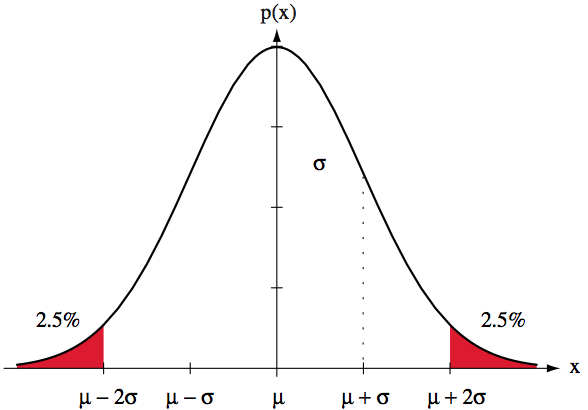
\includegraphics[scale=0.5]{img/gauss.png}
\caption{Distribuzione di Gauss}
\label{gauss}
\end{figure}

\paragraph{Alcune osservazioni}
La funzione è definita su tutto l’asse reale, non è mai né nulla né negativa. Essa è simmetrica rispetto all’asse $y=\mu$  e tende a zero al tendere di $x$ all’infinito. Essa dunque assegna una probabilità a features che hanno range potenzialmente infinito. Inoltre la probabilità assegnata è la stessa per valori equidistanti (sia a destra come a sinistra) da $\mu$. La massima probabilità viene assegnata al valore $\mu$ che si chiama anche valore centrale della distribuzione.\\
Il parametro $\sigma$ serve a determinare quanto è “larga” o “svasata” la campana della gaussiana. Valori grandi per $\sigma$ indicano una “dispersione” notevole dei dati attorno al valore centrale, un valore piccolo invece indica che i dati sono tutti “vicini” al valore centrale. Tale “interpretazione” per il parametro $\sigma$ viene dal fatto che se si calcola l’integrale definito tra $\mu - 2\sigma$ e $\mu + 2\sigma$ si ottiene 0.95. Cioè la popolazione rappresentata dal modello gaussiano si addensa nell’intervallo centrato in $\mu$ e largo $4\sigma$ al $95\%$. Il restante $5\%$ forma le cosidetta “code” della distribuzione.\\

\noindent Trasformazioni lineare di gaussiane: se moltiplico o divido una gaussiana per un valore essa resta sempre una gaussiana, la gaussiana soddisfa il fattore di scaling. Se si sommano le gaussiane si ottiengono mixture di gaussiane, che non sono gaussiane ma distribuzioni di probablità, un insieme di tante campane.\\ 

\noindent Vi è un importante rapporto tra la distribuzione normale e l'entropia\footnote{L'entropia misura la quantità di incertezza o informazione presente in un segnale aleatorio. Da un altro punto di vista l'entropia è la minima complessità descrittiva di una variabile aleatoria, ovvero il limite inferiore della compressione dei dati.}. L'entropia di una distribuzione è calcolata come segue
\begin{equation}
H(p(x)) = - \int p(x) \ln p(x) \ dx
\end{equation}
ed è misurata in \emph{nats}; se invece viene utilizzato il logaritmo di base due, quindi $\log_2$, allora viene misurata in \emph{bit}. L'entropia misura l'incertezza fondamentale nei valori dei punti scelti a caso da una distribuzione.\\

\noindent \emph{Teorema del limite centrale}: L’effetto aggregato ottenuto sommando un grande numero di piccoli contributi random (generati da distribuzioni uniformi) porta ad una distribuzione di Gauss.

\subsection{Distribuzione Multivariata}
La distribuzione Multivariata $d$ dimensionale è scritta come segue
\begin{equation}\label{distribuzioneMultivariata}
p(\mathbf{x}) = \frac{1}{(2\pi)^{d/2} \abs{\mathbf{\Sigma}}^{1/2}} \exp \left [ - \frac{1}{2} (\mathbf{x} - \mathbf{\mu})'  \mathbf{\Sigma}^{-1} (\mathbf{x} - \mathbf{\mu}) \right ]
\end{equation}
dove $\mathbf{x}$ è un vettore colonna, $\mathbf{\mu}$ è il vettore media, $\mathbf{\Sigma}$ è la matrice di covarianza $d \times d$, la matrice di covarianza non è altro che la media dei prodotti degli scarti, $\abs{\mathbf{\Sigma}}$ e $ \mathbf{\Sigma}^{-1}$ sono rispettivamente il determinante e l'inversa. Inoltre denotiamo con $(\mathbf{x} - \mathbf{\mu})' $ la trasposta di $(\mathbf{x} - \mathbf{\mu})$. L'operazione di sottrarre ad ogni $\mathbf{x}$ la propria media $\mathbf{\mu}$ prende il nome di \emph{whitening} (sbiancamento), perchè se si sottrae ad ogni $\mathbf{x}$ la propria media $\mathbf{\mu}$ allora la gaussiana è centrata in 0. Se si vuole ottenere una gaussiana standardizzata bisogna portare la media uguale a zero e la varianza uguale a uno, per fare ciò basta sottrarre la media e dividere per la varianza.
\begin{equation}
Z = \frac{X-\mu}{\sigma}
\end{equation}
La notazione per il prodotto interno è
\begin{equation}
\mathbf{a'b} = \sum_{i=1}^d a_ib_i
\end{equation}
che per semplicità spesso viene chiamato prodotto puntuale. La distribuzione normale spesso viene indicata con $N(\mathbf{\mu, \Sigma})$.
Formalmente la media è calcolata come segue
\begin{equation}
\mathbf{\mu} \equiv \varepsilon[\mathbf{x}] = \int \mathbf{x} p(x) \  d \mathbf{x}
\end{equation}
e la matrice di covarianza 
\begin{equation}
\mathbf{\Sigma} \equiv \varepsilon[(\mathbf{x-\mu)(x-\mu)'}] = \int (\mathbf{x-\mu)(x-\mu)'} p(\mathbf{x})  \  d \mathbf{x}
\end{equation} 
è possibile calcolare il vettore media e la matrice di covarianza anche componente per componente. Nel caso della media, se $x_i$ è la $i$-esima componente di $\mathbf{x}$, se $\mu_i$ è la $i$-esima componente di $\mathbf{\mu}$ e $\sigma_{ij}$ è la $ij$-esima componente di $\mathbf{\Sigma}$ allora
\begin{equation}
\mu_i = \varepsilon[x_i]
\end{equation}
e
\begin{equation}
\sigma_{ij} = \varepsilon[(x_i - \mu_i) (x_j - \mu_j) ]
\end{equation}
Gli elementi $\sigma_{ij}$ della matrice di covarianza hanno una precisa interpretazione. Gli elementi sulla diagonale rappresentano le varianze di ciascuna delle componenti del vettore $\mathbf{x}$. L’elemento $\sigma_{ij}$ se è positivo ci dice che la feature $i$ e la feature $j$ sono correlate positivamente (se una cresce, statisticamente cresce anche l’altra), se è negativo il contrario. Se è nullo ci dice che le feature non sono correlate o che sono statisticamente indipendenti.\\

\noindent I punti si trovano in uno spazio, per semplicità prendiamo lo spazio bidimensionale $x_1$ e $x_2$, come possiamo osservare in figura \ref{gauss1} i campioni giacciono nella nuvola centrata nella media, il luogo dei punti sono degli ellissoidi, dato che stiamo guardando la gaussiana dall'alto.
\begin{figure}
\centering
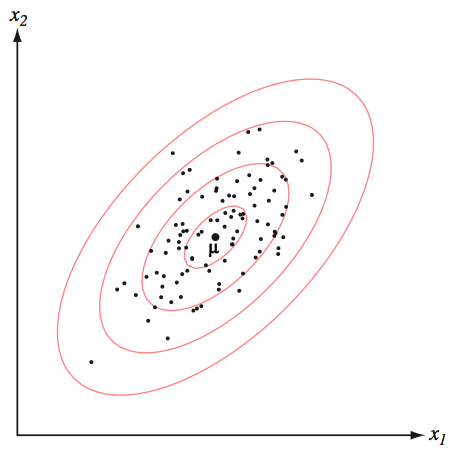
\includegraphics[scale=0.5]{img/gauss1.png}
\caption{Esempio di gaussiana bidimensionale, i campioni giacciono nella nuvola centrata nella media $\mu$}
\label{gauss1}
\end{figure}
Nel caso bidimensionale la gaussiana avrà due varianze, una nella direzione $x_1$ e l'altra nella direzione $x_2$, se le due varianze sono uguali allora la curva di livello è una circonferenza, se invece sono diverse allora è un ellisse. La cosa interessante è che tutti i punti che ricadono nella curva di livello soddisfano questa equazione
\begin{equation}
r^2 = (\mathbf{x- \mu)' \Sigma^{-1} (x- \mu)}
\end{equation}
con $r$ costante. Questa quantità è denominata distanza di \emph{Mahalanobis} da $\mathbf{x}$ a $\mathbf{\mu}$. Se la matrice di covarianza è una matrice diagonale dove sulla diagonale principale ha tutte varianze uguali, allora la distanza diventa euclidea. Un' altra particolarità interessa anche gli autovalori e gli autovettori della matrice di covarianza. Prima di vederla facciamo un breve richiamo sugli Autovalori e Autovettori di una matrice.

\paragraph{Autovalori e Autovettori}
Data la matrice $\mathbf{A}$ gli autovalori si calcolano 
\begin{equation}
\mathbf{A} \mathbf{x} = \lambda \mathbf{x}
\end{equation}
che può essere riscritta come
\begin{equation}
(\mathbf{A} - \lambda \mathbf{I})\mathbf{x} = \mathbf{0}
\end{equation}
dove $\lambda$ sono gli autovalori. Se $\mathbf{A}$ è una matrice quadrata $d \times d$ allora ho $d$ autovalori e $d$ autovettori. Gli autovalori di una matrice danno l'idea dell'energia e sono direttamente proporzionali alle varianze di ogni dimensione, gli autovettori invece sono i vettori che generano un nuovo spazio.\\

\noindent Ritornando alla gaussiana bidimensionale, la cosa interessante è che l'asse maggiore dell'ellisse è uguale alla varianza più grande, mentre l'asse minore è uguale alla varianza più piccola, più precisamente l'asse maggiore è lunga quanto l'autovalore più grande della matrice di covarianza e l'asse minore è lunga quanto l'autovalore più piccolo della matrice di covarianza, inoltre la direzione dell' asse maggiore è l'autovettore corrispondente all'autovalore più grande, mentre la direzione dell'asse minore è l'autovettore corrispondente all'autovalore più piccolo. 

%\paragraph{Trasformazione lineare di funzioni normali e \emph{Whitening (sbiancamento)}}
%Sia $\mathbf{A}$ una matrice $d \times k$ (generalmente è utile pensare a $d$ come più piccolo di $k$). Mediante tale matrice si può trasformare ogni vettore di $k$ componenti in un vettore di $d$ componenti facendo il prodotto $\mathbf{A'x}$. Componendo questa trasformazione con la distribuzione normale $N\mathbf{(\mu,\Sigma})$ si ottiene una nuova distribuzione normale $N(\mathbf{A'\mu, A' \Sigma A})$ come mostrato in figura \ref{sbianc} 
%\begin{figure}
%\centering
%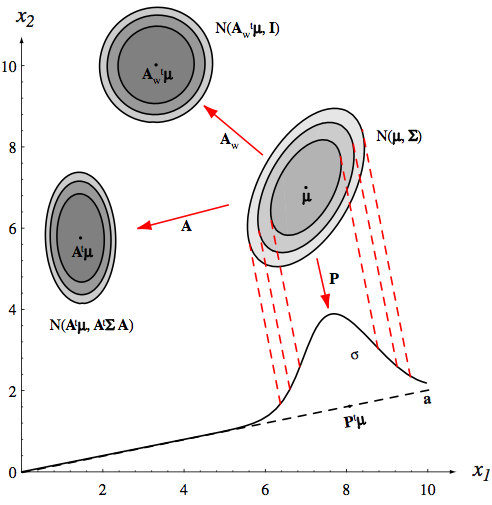
\includegraphics[scale=0.5]{img/sbiancamento.png}
%\caption{Trasformazione lineare}
%\label{sbianc}
%\end{figure}
%Particolarmente utile è la trasformazione con la matrice $k \times k$ \ $\mathbf{A_w}$ (matrice di \emph{whitening} o sbiancamento) che si ottiene come segue:\\ 
%Si calcolano gli autovalori e gli autovettori della matrice di covarianza $\mathbf{\Sigma}$. Si raccolgono gli autovalori in una matrice diagonale $\mathbf{\Lambda}$ e si dispongono nel medesimo ordine come colonne gli autovettori (ortogonali tra loro e normalizzati) in una matrice $\mathbf{\Phi}$. Allora $\mathbf{A_w = \Phi \Lambda}^{-1/2}$.
%La trasformazione con la matrice di \emph{whitening} trasforma la distribuzione gaussiana di partenza (tipicamente ellissoidale orientata in maniera arbitraria nello spazio) in una distribuzione “sferica” con covarianza eguale alla matrice identica. Questo può semplificare in molti casi l’analisi. Ne riparleremo quando affronteremo lo studio della PCA.

\section{Funzioni Discriminanti per la Distribuzione Normale}
Nella sezione \ref{casoMulticategoria} abbiamo visto che un classificatore a minimo tasso di errore può essere espresso usando le funzioni discriminanti
\begin{equation}\label{funzioneDiscriminante}
g_i(\mathbf{x}) = \ln p(\mathbf{x}|\omega_i) + \ln P(\omega_i)
\end{equation}
L'espressione può essere rivalutata se la distribuzione di probabilità $p(\mathbf{x}|\omega_i)$ è una distribuzione multivariata eq. (\ref{distribuzioneMultivariata}). Andando a sostituire all'interno dell' eq. (\ref{funzioneDiscriminante}) e utilizzando le prorpietà dei logaritmi otteniamo:

\begin{equation}\label{fun}
\begin{split}
g_i(\mathbf{x}) &= 
\ln \left \{  
\frac{1}{(2\pi)^{d/2} \abs{\mathbf{\Sigma}_i}^{1/2}} \exp \left [ - \frac{1}{2} (\mathbf{x} - \mathbf{\mu})'  \mathbf{\Sigma}_i^{-1} (\mathbf{x} - \mathbf{\mu}_i) \right ]  
\right \}
+ \ln P(\omega_i) \\
&= \ln \frac{1}{(2\pi)^{d/2} \abs{\mathbf{\Sigma}_i}^{1/2}} + \ln \exp \left [ - \frac{1}{2} (\mathbf{x} - \mathbf{\mu})'  \mathbf{\Sigma}_i^{-1} (\mathbf{x} - \mathbf{\mu}_i) \right ] + \ln P(\omega_i)\\
&= \ln 1 - \ln (2\pi)^{d/2} \abs{\mathbf{\Sigma}_i}^{1/2} - \frac{1}{2} (\mathbf{x} - \mathbf{\mu})'  \mathbf{\Sigma}_i^{-1} (\mathbf{x} - \mathbf{\mu}_i) + \ln P(\omega_i)\\
&= - \left( \frac{d}{2} \ln 2\pi + \frac{1}{2} \ln \abs{\mathbf{\Sigma}} \right) - \frac{1}{2} (\mathbf{x} - \mathbf{\mu})'  \mathbf{\Sigma}_i^{-1} (\mathbf{x} - \mathbf{\mu}_i) + \ln P(\omega_i)\\
&= - \frac{1}{2} (\mathbf{x} - \mathbf{\mu})'  \mathbf{\Sigma}_i^{-1} (\mathbf{x} - \mathbf{\mu}_i) - \frac{d}{2} \ln 2\pi - \frac{1}{2} \ln \abs{\mathbf{\Sigma}} + \ln P(\omega_i) 
%&=  \left [- \frac{1}{2} (\mathbf{x} - \mathbf{\mu}_i)'  \mathbf{\Sigma}_i^{-1} (\mathbf{x} - \mathbf{\mu}_i) \right ] \ln \left ( \frac{1}{(2\pi)^{d/2} \abs{\mathbf{\Sigma}_i}^{1/2}} e \right ) + \ln P(\omega_i) \\
%&= \left [- \frac{1}{2} (\mathbf{x} - \mathbf{\mu}_i)'  \mathbf{\Sigma}_i^{-1} (\mathbf{x} - \mathbf{\mu}_i) \right ] \ln \left ( 2\pi^{-d/2} \right ) + \ln \left ( \abs{\mathbf{\Sigma}_i}^{-1/2} \right ) + \ln e + \ln P(\omega_i)\\
%&= - \frac{1}{2} (\mathbf{x} - \mathbf{\mu}_i)'  \mathbf{\Sigma}_i^{-1} (\mathbf{x} - \mathbf{\mu}_i) -\frac{d}{2} \ln 2\pi - \frac{1}{2} \ln \abs{\mathbf{\Sigma}_i} + \ln P(\omega_i)
\end{split} 
\end{equation}
Adesso possiamo affrontare il problema in tre modi diversi:
\begin{enumerate}
\item Nel primo caso la matrice di covarianza è caratterizzata dalla stessa varianza sulla diagonale principale
\item Nel secondo caso le matrici di covarianza sono uguali per tutte le classi
\item Ne caso generale invece le matrici di covarianza sono diverse per ogni classe
\end{enumerate}

\subsection{Caso 1: $\mathbf{\Sigma_i} = \sigma^2\mathbf{I}$}
Il caso più semplice è quando le caratteristiche sono statisticamente indipendenti e ogni caratteristica ha la stessa varianza $\sigma^2$. In questo caso la matrice di covarianza è diagonale con la stessa varianza sulla diagonale. Geometricamente corrisponde al caso in cui la sezione della gaussiana è una circonferenza, i cluster dell' $i$-esima classe hanno come cento il vettore $\mu_i$. Il calcolo del determinante e dell'inversa è molto semplice, il determinante di una matrice diagonale equivale al prodotto degli elementi sulla diagonale, dato che nel nostro caso gli elementi della diagonale sono tutti uguali allora $\abs{\mathbf{\Sigma_i}} = \sigma^{2d}$, l'inversa $\mathbf{\Sigma_i}^{-1} = (1/\sigma^2)\mathbf{I}$. Inoltre tutti i termini che non sono dipendenti dalle classi possono essere ignorati\footnote{Tutti i termini che non compariranno nei passaggi successivi sono stati omessi perchè sono indipendenti dalle classi.}, quindi andando a sostituire determinante e matrice otteniamo
\begin{equation}
g_i(\mathbf{x}) = -\frac{1}{2}(\mathbf{x} - \mathbf{\mu}_i)' \frac{1}{\sigma^2} (\mathbf{x} - \mathbf{\mu}_i) - \frac{d}{2} \ln 2\pi - \frac{1}{2} \ln \sigma^{2d} + \ln P(\omega_i)
\end{equation}
tutti i termini con la $d$ possono essere ignorati ottenendo 
\begin{equation}
g_i(\mathbf{x}) = -\frac{1}{2\sigma^2} (\mathbf{x} - \mathbf{\mu}_i)' (\mathbf{x} - \mathbf{\mu}_i) + \ln P(\omega_i)
\end{equation}
sviluppando il prodotto  si ottiene
\begin{equation}
g_i(\mathbf{x}) = -\frac{1}{2\sigma^2} \left [ \mathbf{x'x}  - 2\mathbf{\mu}_i' \mathbf{x} + \mu_i' \mu_i\right ] + \ln P(\omega_i)
\end{equation}
anche in questo caso il termine $\mathbf{x'x}$ è lo stesso per tutti gli $i$ e quindi non dipende dalla classe, sviluppando
\begin{equation}
g_i(\mathbf{x}) = \frac{1}{\sigma^2} \mathbf{\mu}_i' \mathbf{x} - \frac{1}{2\sigma^2}\mu_i' \mu_i + \ln P(\omega_i)
\end{equation}
ponendo 
\begin{equation}\label{w}
\mathbf{w}_i = \frac{1}{\sigma^2}\mu_i
\end{equation}
e
\begin{equation}
w_{i0} = - \frac{1}{2\sigma^2} \mu_i' \mu_i + \ln P(\omega_i)
\end{equation}
ottenimo la funzione discriminante lineare
\begin{equation}
g_i(\mathbf{x}) = \mathbf{w}_i'\mathbf{x} + w_{i0}
\end{equation}
che è esattamente una funzione lineare. Viene moltiplicato il vettore $\mathbf{w}_i$ che dipende esclusivamente dalla classe $i$-esima, infatti è uguale proprio al centroide della classe $i$-esima (dalla \ref{w}), mentre $w_{i0}$ è un fattore di traslazione chiamato anche \emph{bias}. Si può dire che il problema è \emph{biased} oppure \emph{unbiased}, cioè condizionato oppure non condizionato, è condizionato se si attribuiscono delle conoscenze a priori che si hanno, infatti il \emph{bias} dipende proprio dalla probabilità a priori della classe. Se invece non si considerano le probabilità a priori allora la stima è \emph{unbiased}.\\
Un classificatore che è una funzione discriminante lineare è chiamato \emph{linear machine}. 
Possiamo dire che la superficie di decisione di un classificatore lineare è un iperpiano definito dall'equazione $g_i(\mathbf{x}) = g_j(\mathbf{x})$. Per un caso particolare l'equazione può essere scritta come
\begin{equation}
\mathbf{w}'(\mathbf{x - x}_0) = 0
\end{equation}
dove
\begin{equation}
\mathbf{w} = \mu_i - \mu_j
\end{equation}
e
\begin{equation}\label{iperpiano}
\mathbf{x}_0 = \frac{1}{2}(\mu_i - \mu_j) - \frac{\sigma^2}{\norma{\mu_i - \mu_j}^2} \ln \frac{P(\omega_i)}{P(\omega_j)}(\mu_i - \mu_j) 
\end{equation}
dove
\begin{equation}
\norma{\mu_i - \mu_j}^2 =  (\mathbf{x} - \mathbf{\mu}_i)' (\mathbf{x} - \mathbf{\mu}_i) 
\end{equation}
L'equazione \ref{iperpiano} definisce l'iperpiano passante per il punto $\mathbf{x}_0$ e ortagonale al vettore $\mathbf{w}$. Poichè  $\mathbf{w} = \mu_i - \mu_j$, l'iperpiano che separa $\mathcal{R}_1 \  \text{e} \  \mathcal{R}_2$ è ortogonale alla linea che collega le medie. Se $P(\omega_i) = P(\omega_j)$ allora il secondo temine dell'equazione \ref{iperpiano} svanisce, così il punto $\mathbf{x}_0$ si trova giusto al centro tra le due medie, e l'iperpiano è la bisettrice perpendicolare tra le medie (Fig. \ref{fig_iperpiano}). 
\begin{figure}
\centering
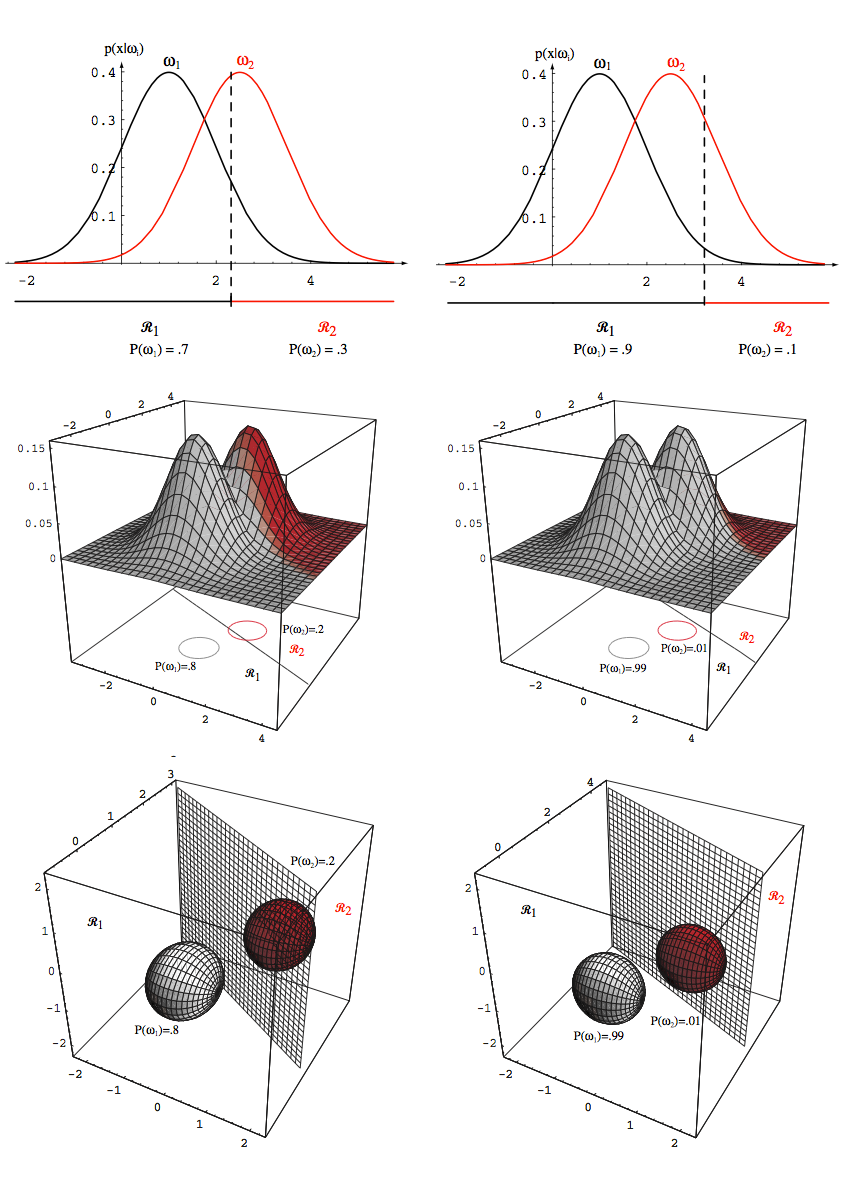
\includegraphics[scale=0.55]{img/hyperpiano.png}
\caption{Quando le probabilità a priori cambiano, la regione di decisione shifta}
\label{fig_iperpiano}
\end{figure}
Se $P(\omega_i) \neq P(\omega_j)$, il punto $\mathbf{x}_0$ si muove fra le due medie. Se invece le probabilità a priori $P(\omega_i)$ sono uguali per tutte le $c$ classi, allora anche il termine $\ln P(\omega_i)$ può essere ignorato. Per classificare un vettore delle caratteristiche $\mathbf{x}$, si misura la distanza euclidea $\norma{\mathbf{x} - \mu_i}$ da ogni vettore delle medie $\mu_i$ delle $c$ classi e viene assegnato $\mathbf{x}$ alla classe più vicina. Per questo motivo è anche detto \emph{classificatore a minima distanza}. 

\subsection{Caso 2: $\mathbf{\Sigma}_i = \mathbf{\Sigma}$}
Un altro semplice caso è quando le matrici di covarianza per tutte le classi sono uguali. Geometricamente corrisponde alla situazione in cui la sezione della gaussiana vista dall'alto corrisponde ad un ellissoide, tutte della stessa diemensione e forma, ognuna centrata nel vettore delle medie $\mu_i$. Anche in questo caso sia $\abs{\mathbf{\Sigma}_i}$ che $(d/2) \ln 2\pi$ nell'equazione \ref{fun} non dipendono dalle classi e quindi possono essere ignorati, come prima la semplificazione porta alla seguente funzione discriminante
\begin{equation}
g_i(\mathbf{x})  =\frac{1}{2}(\mathbf{x} - \mu_i)' \mathbf{\Sigma}^{-1}(\mathbf{x} - \mu_i) + \ln P(\omega_i)
\end{equation}
come si può osservare anche in questo caso il classificatore è lineare, quindi è un hyperpiano.
Se le probabilità a priori $P(\omega_i)$ sono uguali per tutte le $c$ classi, allora anche in questo caso il temine $\ln P(\omega_i)$ può essere ignorato. Anche in questo caso la regola di decisione risulta essere davvero semplice: Per classificare il vettore $\mathbf{x}$ si calcola la distanza di \emph{Mahalanobis} $(\mathbf{x} - \mu_i)' \mathbf{\Sigma}^{-1}(\mathbf{x}- \mu_i)$ da ogni vettore delle medie, e si assegna $\mathbf{x}$ a quello più vicino. Come prima se ci si trova di fronte a probabilità a priori diverse per ogni classe allora queste condizionano la decisione verso la categoria che ha pobabilità più alta. 

\subsection{Caso 3: $\mathbf{\Sigma}_i$ = arbitrario}
Nel caso generale di una distribuzione normale multivariata, allora le matrici di covarianza sono diverse per ogni classe. L'unico termine che può essere ignorato è $(d/2) \ln 2\pi$ e la funzione discriminante risulta essere una quadrica. Ovvero una forma qualsiasi che rappresenta esattamente un classificatore chiamato quadratico, in tal caso le superfici di decisione non sono iperpiani ma sono delle iperquadriche, paraboloidi che si intersecano. 

\section{Probabilità di errore ed integrali}
Consideriamo prima il caso a due categoria e supponiamo che il classificatore abbia separato le due regioni $\mathcal{R}_1$ e $\mathcal{R}_2$. Ci sono due modi nel quale il classificatore può commettere un errore: quello di assegnare l'osservazione $\mathbf{x}$ alla regione $\mathcal{R}_2$ quando il suo vero stato della natura doveva essere $\omega_1$ e quello di assegnare l'osservazione $\mathbf{x}$ alla regione $\mathcal{R}_1$ quando il suo vero stato della natura doveva essere $\omega_2$. Poichè questi eventi sono mutuamente esclusivi allora la probabilità di errore è calcolata come segue
\begin{equation}
\begin{split}
P(error) &= P(\mathbf{x} \in \mathcal{R}_2, \omega_1) + P(\mathbf{x} \in \mathcal{R}_1, \omega_2) \\
&= P(\mathbf{x} \in \mathcal{R}_2|\omega_1) P(\omega_1) + P(\mathbf{x} \in \mathcal{R}_1|\omega_2) P(\omega_2)\\
&= \int_{\mathcal{R}_2} p(\mathbf{x}|\omega_1) P(\omega_1) \ d\mathbf{x} + \int_{\mathcal{R}_1} p(\mathbf{x}|\omega_2) P(\omega_2) \ d\mathbf{x}
\end{split}
\end{equation}

\noindent Il risultato nel caso monodimensionale è illustrato in figura \ref{errore}. I due integrali calcolati sono rappresentati dall'area rosa e grigia. Dato che il punto di decisione è $x^*$ la probabilità di errore non è minima. In particolare l'aria marcata con il bordo rosso è l'errore riducibile che può essere ridotto spostando il punto di decisione verso $x_B$. Nel caso multicategoria, invece è più semplice calcolare la probabilità di correttezza nel modo seguente
\begin{equation}
\begin{split}
P(correct) &= P(\mathbf{x} \in \mathcal{R}_i, \omega_i) \\
&= \sum_{i=1}^c P(\mathbf{x} \in \mathcal{R}_i | \omega_i) P(\omega_i) \\
&= \sum_{i=1}^c \int_{\mathcal{R}_i} p(\mathbf{x}|\omega_i)P(\omega_i) \ d\mathbf{x}
\end{split}
\end{equation} 
In questo caso si fa uso della sommatoria perchè le classi sono $c$, quindi un insieme finito e numerabile, quindi la probabiità di appartenenza di ogni classe è discreta, invece è continua la densità di probabilità. 


\begin{figure}
\centering
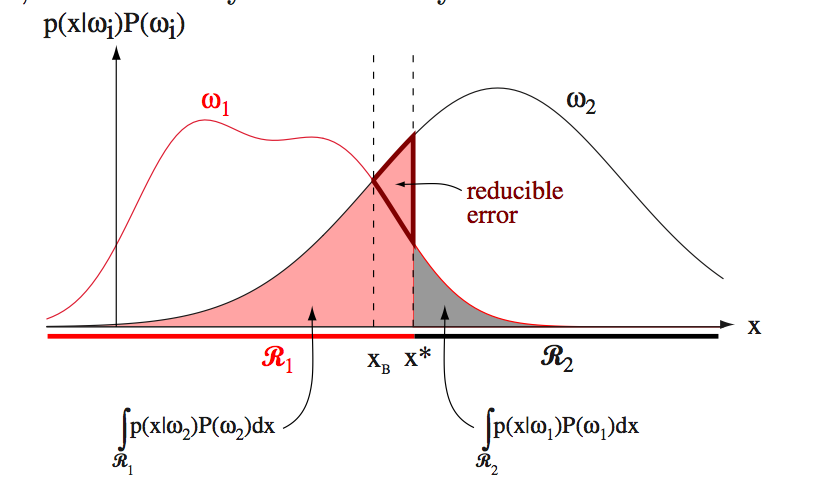
\includegraphics[scale=0.45]{img/errore.png}
\caption{Probabilità di errore nel caso il punto di decisione sia $x^*$. L'area rosa corrisponde alla probabilità di errore di decidere lo stato $\omega_1$ quando dovrebbe essere $\omega_2$; l'area grigia corrisponde alla situazione opposta.}
\label{errore}
\end{figure}

\subsection{Receiver Operating Characteristic (R.O.C.)}
Osservando al figura \ref{errore1} possiamo distinguere quattro aree
\begin{itemize}
\item $P(x > x^* | x \in \omega_2)$: La probabilità che l'osservazione venga classificata come $\omega_2$ e appartiene alla classe $\omega_2$, quindi una classificazione esatta che viene indicata in genere con i seguenti termini: \emph{hit} o \emph{true positive}
\item $P(x > x^* | x \in \omega_1)$:  La probabilità che l'osservazione venga classificata come $\omega_2$ e appartiene alla classe $\omega_1$, quindi una classificazione non corretta che viene indicata in genere con i seguenti termini: \emph{false alarm} o \emph{false positive} 
\item $P(x < x^* | x \in \omega_2)$:  La probabilità che l'osservazione venga classificata come $\omega_1$ e appartiene alla classe $\omega_2$, quindi una classificazione non corretta che viene indicata in genere con i seguenti termini: \emph{miss} o \emph{false negative}
\item $P(x < x^* | x \in \omega_1)$:  La probabilità che l'osservazione venga classificata come $\omega_1$ e appartiene alla classe $\omega_1$, quindi una classificazione corretta che viene indicata in genere con i seguenti termini: \emph{correct rejection} o \emph{true negative}
\end{itemize}
\begin{figure}
\centering
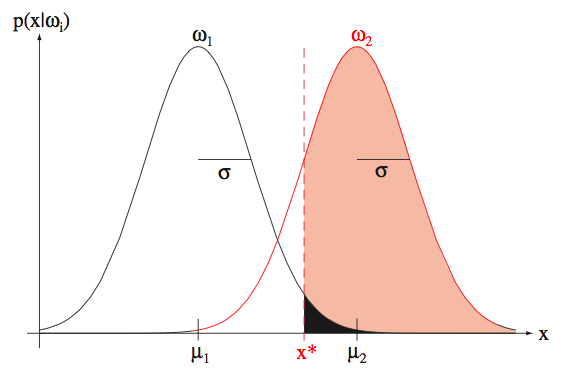
\includegraphics[scale=0.5]{img/errore1.png}
\caption{}
\label{errore1}
\end{figure}
Le curve di ROC è un plot che si basa sui valori ottenuti dalla matrice di confusione, quindi in un primo passo si calcola la matrice di confusione.
\[
\left(
\begin{array}{cc}
 VP & FP \\
 FN & VN 
\end{array}
\right)
\]
ROC sta per \emph{Receiver Operating Characteristic}, sostanzialmente ci aspettiamo che questo sistema segnali correttamente o non correttamente e vogliamo misurare il comportamento, cioè la rilevazione di un oggetto oppure il verificarsi di un evento. La ROC (Fig. \ref{roc}) è una curva che viene plottata nello spazio bidimensionale, sull'asse delle ascisse viene riportato il \emph{false positive rate} oppure più comunemente la Specificità, cioè il rapporto dei casi classificati come corretti ma appartenenti ad una classe diversa \emph{false positive}, rispetto al numero totale dei casi negativi, quindi
\begin{equation}
S_p = \frac{FP}{FP+VN}
\end{equation}
invece sull'asse delle ordinate abbiamo il \emph{true positive rate}, oppure più comunemente la Sensibilità cioè il rapporto dei casi positivi classificati come positivi ed il numero totale dei casi positivi, quindi
\begin{equation}
S_e = \frac{VP}{VP+FN}
\end{equation}
Il risultato desiderato è quello che il classificatore ci desse il  massimo per il \emph{true positive rate} (sensibilità) mentre il \emph{false positive rate} (specificità) sia minimo, quindi ci si aspetta il grafico mostrato in figura \ref{roc}.
\begin{figure}
\centering
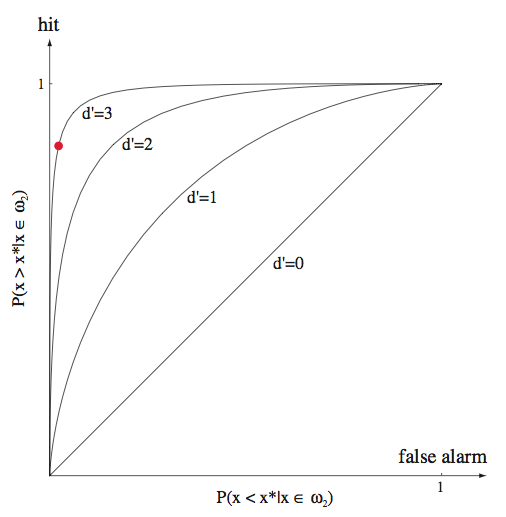
\includegraphics[scale=0.5]{img/roc.png}
\caption{}
\label{roc}
\end{figure}
L’analisi ROC viene effettuata attraverso lo studio della funzione che  lega la probabilità di ottenere un risultato vero-positivo nella classe dei pattern da classificare come veri (ossia la sensibilità) alla probabilità di ottenere un risultato falso-positivo nella classe dei pattern da classificare come falsi(ossia specificità). In altre parole, vengono studiati i rapporti fra allarmi veri (hit rate) e falsi allarmi. La capacità discriminante di un test, ossia la sua attitudine a separare propriamente la popolazione in studio è proporzionale all’estensione dell’area sottesa alla curva ROC (Area Under Curve, AUC). Nel caso di un test perfetto, ossia che non restituisce alcun falso positivo né falso negativo (capacità discriminante = $100\%$), la AUC passa attraverso le coordinate {0;1} ed il suo valore corrisponde all’area dell’intero quadrato delimitato dai punti di coordinate (0,0), (0,1), (1,0) (1,1), che assume valore 1 corrispondendo ad una probabilità del $100\%$ di una corretta classificazione. 


%%%%%%%%%%%%%%%%%%%%% chapter.tex %%%%%%%%%%%%%%%%%%%%%%%%%%%%%%%%%
%
% sample chapter
%
% Use this file as a template for your own input.
%
%%%%%%%%%%%%%%%%%%%%%%%% Springer-Verlag %%%%%%%%%%%%%%%%%%%%%%%%%%

\chapter{Chapter Heading}
\label{intro} % Always give a unique label
% use \chaptermark{}
% to alter or adjust the chapter heading in the running head

Your text goes here. Separate text sections with the standard \LaTeX\
sectioning commands.

\section{Section Heading}
\label{sec:1}
% Always give a unique label
% and use \ref{<label>} for cross-references
% and \cite{<label>} for bibliographic references
% use \sectionmark{}
% to alter or adjust the section heading in the running head
Your text goes here. Use the \LaTeX\ automatism for your citations
\cite{monograph}.

\subsection{Subsection Heading}
\label{sec:2}
Your text goes here.

\begin{equation}
\vec{a}\times\vec{b}=\vec{c}
\end{equation}

\subsubsection{Subsubsection Heading}
Your text goes here. Use the \LaTeX\ automatism for cross-references as
well as for your citations, see Sect.~\ref{sec:1}.

\paragraph{Paragraph Heading} %
Your text goes here.

\subparagraph{Subparagraph Heading.} Your text goes here.%
%
\index{paragraph}
% Use the \index{} command to code your index words
%
% For tables use
%
\begin{table}
\centering
\caption{Please write your table caption here}
\label{tab:1}       % Give a unique label
%
% For LaTeX tables use
%
\begin{tabular}{lll}
\hline\noalign{\smallskip}
first & second & third  \\
\noalign{\smallskip}\hline\noalign{\smallskip}
number & number & number \\
number & number & number \\
\noalign{\smallskip}\hline
\end{tabular}
\end{table}
%
%
% For figures use
%
\begin{figure}
\centering
% Use the relevant command for your figure-insertion program
% to insert the figure file.
% For example, with the option graphics use
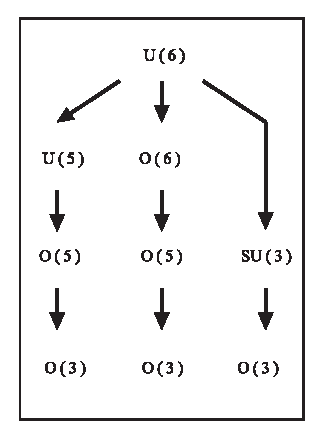
\includegraphics[height=4cm]{figure.eps}
%
% If not, use
%\picplace{5cm}{2cm} % Give the correct figure height and width in cm
%
\caption{Please write your figure caption here}
\label{fig:1}       % Give a unique label
\end{figure}
%
% For built-in environments use
%
\begin{theorem}
Theorem text goes here.
\end{theorem}
%
% or
%
\begin{lemma}
Lemma text goes here.
\end{lemma}
%
%
% Problems or Exercises should be sorted chapterwise
\section*{Problems}
\addcontentsline{toc}{section}{Problems}
%
% Use the following environment.
% Don't forget to label each problem;
% the label is needed for the solutions' environment
\begin{prob}
\label{prob1}
The problem\footnote{Footnote} is described here. The
problem is described here. The problem is described here.
\end{prob}

\begin{prob}
\label{prob2}
\textbf{Problem Heading}\\
(a) The first part of the problem is described here.\\
(b) The second part of the problem is described here.
\end{prob}



%

%%%%%%%%%%%%%%%%%%%%%% chapter.tex %%%%%%%%%%%%%%%%%%%%%%%%%%%%%%%%%
%
% sample chapter
%
% Use this file as a template for your own input.
%
%%%%%%%%%%%%%%%%%%%%%%%% Springer-Verlag %%%%%%%%%%%%%%%%%%%%%%%%%%

\chapter{Chapter Heading}
\label{intro} % Always give a unique label
% use \chaptermark{}
% to alter or adjust the chapter heading in the running head

Your text goes here. Separate text sections with the standard \LaTeX\
sectioning commands.

\section{Section Heading}
\label{sec:1}
% Always give a unique label
% and use \ref{<label>} for cross-references
% and \cite{<label>} for bibliographic references
% use \sectionmark{}
% to alter or adjust the section heading in the running head
Your text goes here. Use the \LaTeX\ automatism for your citations
\cite{monograph}.

\subsection{Subsection Heading}
\label{sec:2}
Your text goes here.

\begin{equation}
\vec{a}\times\vec{b}=\vec{c}
\end{equation}

\subsubsection{Subsubsection Heading}
Your text goes here. Use the \LaTeX\ automatism for cross-references as
well as for your citations, see Sect.~\ref{sec:1}.

\paragraph{Paragraph Heading} %
Your text goes here.

\subparagraph{Subparagraph Heading.} Your text goes here.%
%
\index{paragraph}
% Use the \index{} command to code your index words
%
% For tables use
%
\begin{table}
\centering
\caption{Please write your table caption here}
\label{tab:1}       % Give a unique label
%
% For LaTeX tables use
%
\begin{tabular}{lll}
\hline\noalign{\smallskip}
first & second & third  \\
\noalign{\smallskip}\hline\noalign{\smallskip}
number & number & number \\
number & number & number \\
\noalign{\smallskip}\hline
\end{tabular}
\end{table}
%
%
% For figures use
%
\begin{figure}
\centering
% Use the relevant command for your figure-insertion program
% to insert the figure file.
% For example, with the option graphics use
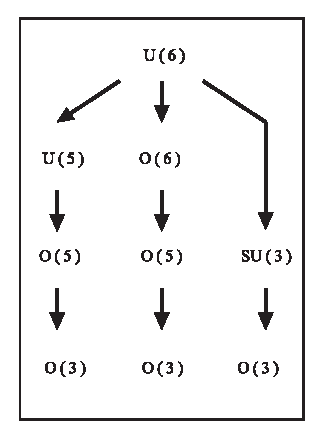
\includegraphics[height=4cm]{figure.eps}
%
% If not, use
%\picplace{5cm}{2cm} % Give the correct figure height and width in cm
%
\caption{Please write your figure caption here}
\label{fig:1}       % Give a unique label
\end{figure}
%
% For built-in environments use
%
\begin{theorem}
Theorem text goes here.
\end{theorem}
%
% or
%
\begin{lemma}
Lemma text goes here.
\end{lemma}
%
%
% Problems or Exercises should be sorted chapterwise
\section*{Problems}
\addcontentsline{toc}{section}{Problems}
%
% Use the following environment.
% Don't forget to label each problem;
% the label is needed for the solutions' environment
\begin{prob}
\label{prob1}
The problem\footnote{Footnote} is described here. The
problem is described here. The problem is described here.
\end{prob}

\begin{prob}
\label{prob2}
\textbf{Problem Heading}\\
(a) The first part of the problem is described here.\\
(b) The second part of the problem is described here.
\end{prob}



%

%\appendix
%\include{appendix}

%%%%%%%%%%%%%%%%%%%%%%%% part.tex %%%%%%%%%%%%%%%%%%%%%%%%%%%%%%%%%%
%
% sample part title
%
% Use this file as a template for your own input.
%
%%%%%%%%%%%%%%%%%%%%%%%% Springer-Verlag %%%%%%%%%%%%%%%%%%%%%%%%%%


\part{Sistemi Adattivi e Reti Neurali}

%%%%%%%%%%%%%%%%%%%%% chapter.tex %%%%%%%%%%%%%%%%%%%%%%%%%%%%%%%%%
%
% sample chapter
%
% Use this file as a template for your own input.
%
%%%%%%%%%%%%%%%%%%%%%%%% Springer-Verlag %%%%%%%%%%%%%%%%%%%%%%%%%%

\chapter{Chapter Heading}
\label{intro} % Always give a unique label
% use \chaptermark{}
% to alter or adjust the chapter heading in the running head

Your text goes here. Separate text sections with the standard \LaTeX\
sectioning commands.

\section{Section Heading}
\label{sec:1}
% Always give a unique label
% and use \ref{<label>} for cross-references
% and \cite{<label>} for bibliographic references
% use \sectionmark{}
% to alter or adjust the section heading in the running head
Your text goes here. Use the \LaTeX\ automatism for your citations
\cite{monograph}.

\subsection{Subsection Heading}
\label{sec:2}
Your text goes here.

\begin{equation}
\vec{a}\times\vec{b}=\vec{c}
\end{equation}

\subsubsection{Subsubsection Heading}
Your text goes here. Use the \LaTeX\ automatism for cross-references as
well as for your citations, see Sect.~\ref{sec:1}.

\paragraph{Paragraph Heading} %
Your text goes here.

\subparagraph{Subparagraph Heading.} Your text goes here.%
%
\index{paragraph}
% Use the \index{} command to code your index words
%
% For tables use
%
\begin{table}
\centering
\caption{Please write your table caption here}
\label{tab:1}       % Give a unique label
%
% For LaTeX tables use
%
\begin{tabular}{lll}
\hline\noalign{\smallskip}
first & second & third  \\
\noalign{\smallskip}\hline\noalign{\smallskip}
number & number & number \\
number & number & number \\
\noalign{\smallskip}\hline
\end{tabular}
\end{table}
%
%
% For figures use
%
\begin{figure}
\centering
% Use the relevant command for your figure-insertion program
% to insert the figure file.
% For example, with the option graphics use
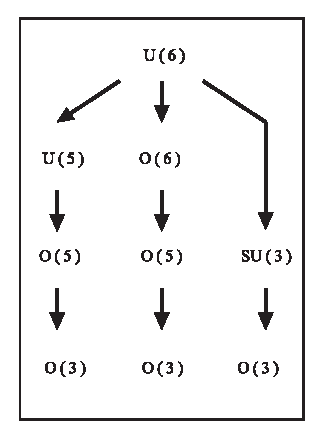
\includegraphics[height=4cm]{figure.eps}
%
% If not, use
%\picplace{5cm}{2cm} % Give the correct figure height and width in cm
%
\caption{Please write your figure caption here}
\label{fig:1}       % Give a unique label
\end{figure}
%
% For built-in environments use
%
\begin{theorem}
Theorem text goes here.
\end{theorem}
%
% or
%
\begin{lemma}
Lemma text goes here.
\end{lemma}
%
%
% Problems or Exercises should be sorted chapterwise
\section*{Problems}
\addcontentsline{toc}{section}{Problems}
%
% Use the following environment.
% Don't forget to label each problem;
% the label is needed for the solutions' environment
\begin{prob}
\label{prob1}
The problem\footnote{Footnote} is described here. The
problem is described here. The problem is described here.
\end{prob}

\begin{prob}
\label{prob2}
\textbf{Problem Heading}\\
(a) The first part of the problem is described here.\\
(b) The second part of the problem is described here.
\end{prob}



%


\backmatter%%%%%%%%%%%%%%%%%%%%%%%%%%%%%%%%%%%%%%%%%%%%%%%%%%%%%%%

\chapter*{Solutions}
\addcontentsline{toc}{chapter}{Solutions}
\markboth{Solutions}{Solutions}

\section*{Problems of Chapter~\ref{intro}}

\begin{sol}{prob1}
The solution is revealed here.
\end{sol}


\begin{sol}{prob2}
\textbf{Problem Heading}\\
(a) The solution of first part is revealed here.\\
(b) The solution of second part is revealed here.
\end{sol}


%%%%%%%%%%%%%%%%%%%%%%%% referenc.tex %%%%%%%%%%%%%%%%%%%%%%%%%%%%%%
% sample references
% "computer science"
%
% Use this file as a template for your own input.
%
%%%%%%%%%%%%%%%%%%%%%%%% Springer-Verlag %%%%%%%%%%%%%%%%%%%%%%%%%%

%
% BibTeX users please use
% \bibliographystyle{}
% \bibliography{}
%
% Non-BibTeX users please use
\begin{thebibliography}{99.}
%
% and use \bibitem to create references.
%
% Use the following syntax and markup for your references
%
% Monographs
\bibitem{monograph} Kajan E (2002)
Information technology encyclopedia and acronyms. Springer, Berlin
Heidelberg New York

% Contributed Works
\bibitem{contribution} Broy M (2002) Software engineering -- From
auxiliary to key technologies. In: Broy M, Denert E (eds)
Software Pioneers. Springer, Berlin Heidelberg New York

% Journal
\bibitem{journal} Che M, Grellmann W, Seidler S (1997)
Appl Polym Sci 64:1079--1090

% Theses
\bibitem{thesis} Ross DW (1977) Lysosomes and storage diseases. MA
Thesis, Columbia University, New York

\end{thebibliography}

\printindex

%%%%%%%%%%%%%%%%%%%%%%%%%%%%%%%%%%%%%%%%%%%%%%%%%%%%%%%%%%%%%%%%%%%%%%

\end{document}





